% !TeX document-id = {7d02b5cb-bef5-4e3c-b3ad-71af769d0806}
\documentclass{beamer}
\usepackage{authblk}
\usepackage{graphicx}
\usepackage{csquotes}
\usepackage{pgfplots}
\usepackage{amsmath}
\usepackage{wrapfig}
\usepackage{siunitx}
\usepackage{minted}
\usepackage{subcaption}
\usepackage{array}
\usepackage{varwidth}

% !TeX TXS-program:compile = txs:///pdflatex/[--shell-escape]

\usetheme{CambridgeUS}
\usebeamercolor{rose}

\pgfplotsset{width=10cm,compat=1.9}
\setlength{\parindent}{0pt}

\title{Development report}
\author[Author]{Leonardo Pavarino s269609}
\institute [Politecnico di Torino]% (optional)
{ 
	Leonardo Pavarino s269609\\
	Open and virtualized networks\\
	Politecnico di Torino  
}
\affil{Open and Virtualized networks}
\subject{Open and virtualized Networks}
\date[2022]{}


\begin{document}
	\maketitle
	\section{Introduction}
	\begin{frame}{Introduction}
		During this course I was asked to develop a digital twin of a fiber network.\\
		This tween had to be able to simulate traffic through the network and so allow for optimized pathing either by selecting the better path by SNR or latency using a virtual circuits' architecture.\\
		The simulated network is the a partly disaggregated and not a fully disaggregated network since the fibers spanns and the ampliers are considered as a single network entity: OLSs, and are not independently accessible by the network controller.
	\end{frame}
	\section{The network infastructure}
	\begin{frame}{The network}
		The network I had to emulate was mad up of 5 nodes connected by multimode fiber lines. Each line in the picture below represents two fiber lines, one for each direction.
		\begin{figure}
			\centering
			\label{fig:network}
			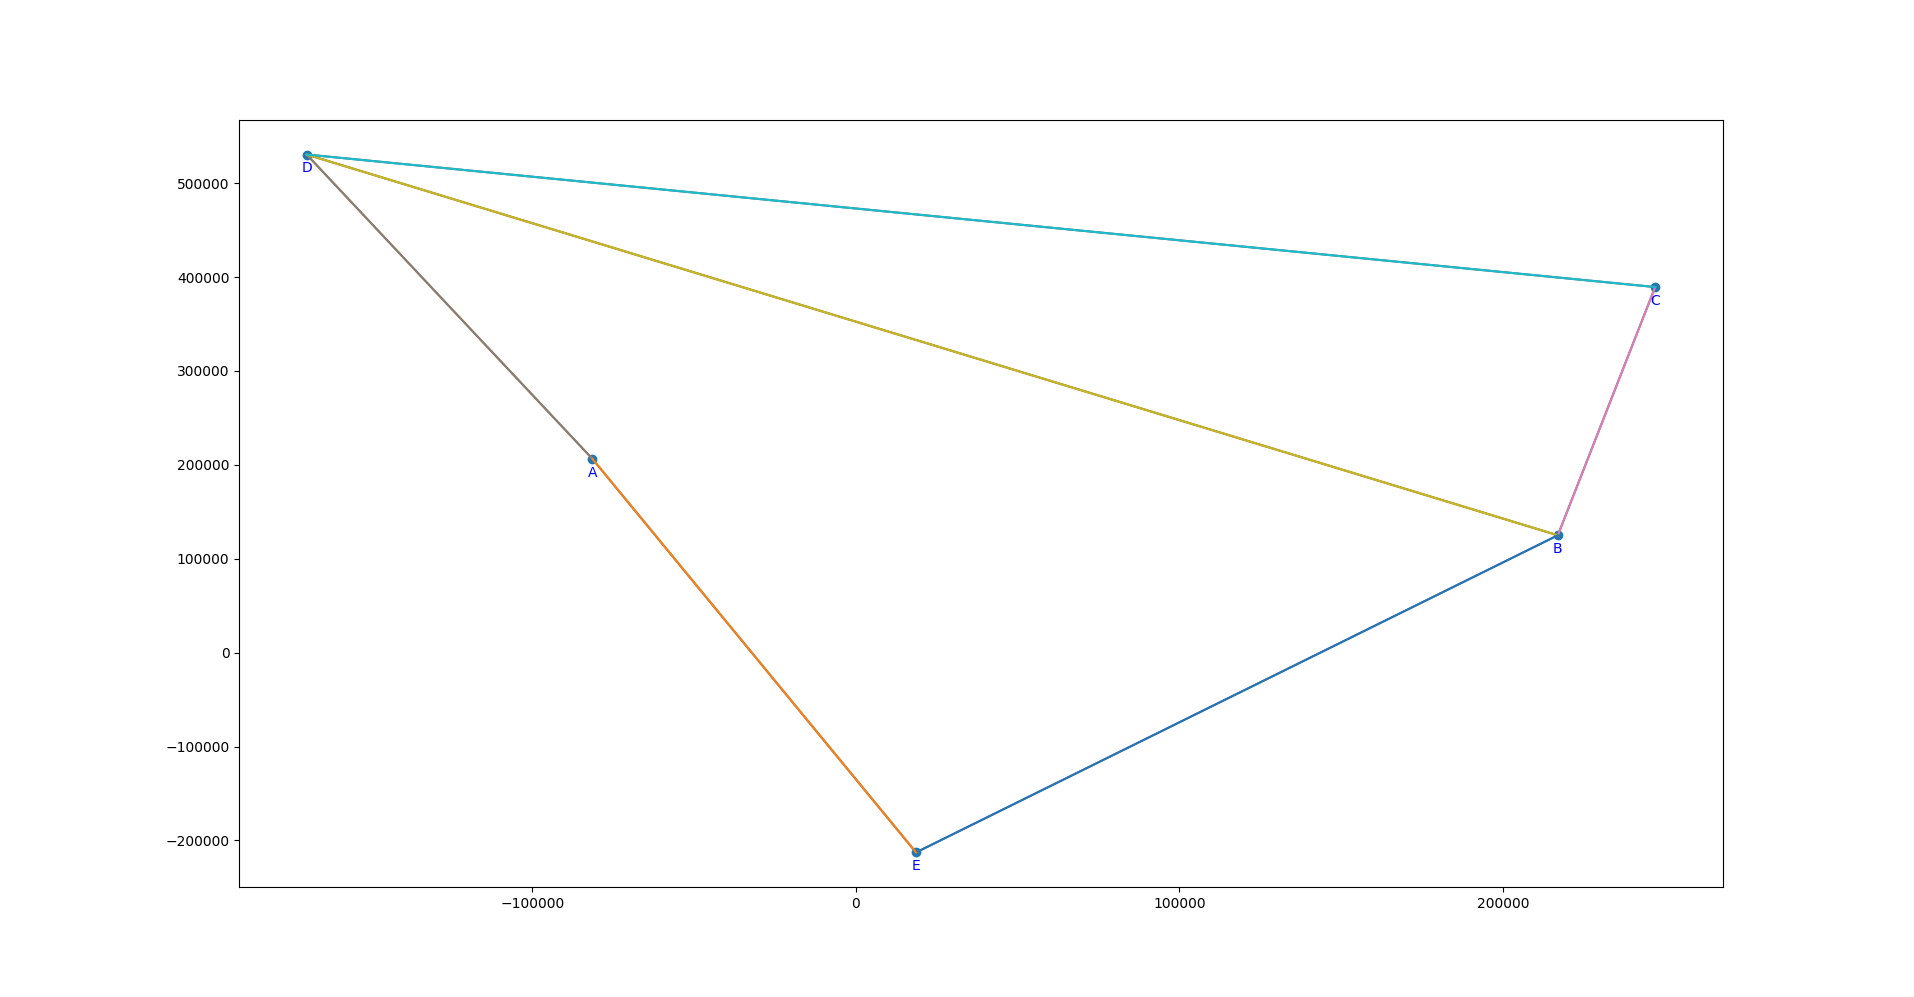
\includegraphics[width=\linewidth]{Pictures/my network.png}
			%\caption{Image of the network in 269609.json}
		\end{figure}
	\end{frame}
	\section{Classes Outline}
	\subsection{Signal information}
	\label{slide:SigInf}
	\begin{frame}{Signal information outline}
		This class represents a signal propating through the network.
	\end{frame}
	\begin{frame}{Signal information outline}
		This class has the following attributes:
		\begin{itemize}
			\item Signal Power: the power of the signal.
			\item Noise Power: the power of the noise.
			\item Latency: the latency the signal accumalated since its transmission.
			\item Path: a list of nodes the signal is going to travel through to reach its destination.
		\end{itemize}
	\end{frame}
	\begin{frame}[fragile]
		It also implements a method to calculate the signal to noise ratio in dB using the following formula:
		\begin{equation}
			SNR=10 \cdot \log_{10} \left( \frac{P_{signal}}{P_{noise}} \right)
		\end{equation} \pause
		in the following way:
		\begin{minted}[frame=lines,
			framesep=2mm,
			baselinestretch=1.2,
			fontsize=\footnotesize,
			linenos]{python}
def get_signal_noise_ration(self) -> float :
	return 10 * (log10(self.signal_power) - \
				log10(self.noise_power))
		\end{minted}
	\end{frame}
	\subsection{Light path}
	\begin{frame}{Light path outline}
		This class extends the class Signal Information(\ref{slide:SigInf}) and represents a light path that propagates thorugh the network at a given wavelength. \\
		%it is similar to a virtual circuit established in the network as the resources like channels are assigned to it and requires messages to be exanged to initialize it in a process that can last up to some minutes.
		It is a dedicated optical channel or a virtual circtuit for which resources are allocated untill it is closed; For this reason it requires messages to be exanchange between nodes so that the required resources can be allocated, it can take up to a few minutes for it be established.
	\end{frame}
	\begin{frame}{Light path outline}
		The light path class extends the Signal Information(\ref{slide:SigInf}) class with the following attribute:
		\begin{itemize}
			\item channel: the channel in the optical fiber the signal is traveling in.
		\end{itemize}
	\end{frame}
	\subsection{Node}
	\begin{frame}{Node outline}
		This class reprensents a ROADM (Reconfigurable add/drop multiplexer) which is switch that is also able to remove and add the local traffic from and to the fiber network.\pause \\
		It's switching and add/drop matricies can be reconfigured dynamically by the network controller.
	\end{frame}
	\begin{frame}{Node outline}
		This nodes are also CDC (Colorless, Directionless and Contensionless) switches: \pause
		\begin{itemize}
			\item Colorless: any input mode can be addressed to any output fiber, indipendently from its wavelenght (color).\pause
			\item Directionless: any input mode can be addressed to any output fiber, indipendently from its direction.\pause
			\item Contentionless: these operations can be done for every input load, so no traffic-dependent contention is introduced.
		\end{itemize}
	\end{frame}
	\begin{frame}{Node Attributes}
		The node class represents a node in the network, it has the following attributes:
		\begin{itemize}
			\item Label: the name of the node.
			\item Position: the position of the node.
			\item Connected Nodes: a list that contains the labels of the other nodes that are reachable.
			\item Successive: a dictionary that contains the references to the lines and are identified by the label of the node at the other end.
			\item Transceiver: a string which indicates which transceiver technology is utilised by the node.
		\end{itemize}
	\end{frame}
	\begin{frame}[fragile]{propagate}
		It also implements the method propagate which accepts a Signal\_Infromation object, it extracs the next node in the path and then calls the method propagate on the line connected to it.
		\begin{minted}[frame=lines,
			framesep=2mm,
			baselinestretch=1.2,
			fontsize=\footnotesize,
			linenos]{python}
def propagate(self, signal : Signal_information):
	next_node = signal.update_path()
	if(next_node in self.connected_node):
	signal.signal_power = self.successive[next_node].
			optimized_launch_power()   # set the optimized 
					#launch power of the signal
	self.successive[next_node].propagate(signal)                                # for this line

		\end{minted}
	\end{frame}
	\begin{frame}{Transceivers}
		The nodes in the system also posses three possible types of transceivers which determin the maximum speeds of transmissions:
		\begin{itemize}
			\item Fixed rate: 100 Gb/s achivable if a certain GSNR threshold was reached, otherwise no comunication was possible.
			\begin{center}
				$R_b = \begin{cases}
					$0 Gb/s	 \hspace{21px} if $GSNR < 2 \cdot erfcinv^2\left(2 \cdot BERT_t \right) \cdot \frac{R_s}{B_n} \\
					$100 Gb/s \hspace{10px} if $GSNR \geq 2 \cdot erfcinv^2\left(2 \cdot BERT_t \right) \cdot \frac{R_s}{B_n}
				\end{cases} $
			\end{center}
			\item Flex rate: added other two threshholds for 200 Gb/s and 400 Gb/s speeds.
			\begin{center}
				\begin{tiny}
					$R_b = \begin{cases}
					$0 Gb/s	 \hspace{21px} if $GSNR < 2 \cdot erfcinv^2\left(2 \cdot BERT_t \right) \cdot \frac{R_s}{B_n} \\
					$100 Gb/s \hspace{10px} if $  2 \cdot erfcinv^2\left(2 \cdot BERT_t \right) \cdot \frac{R_s}{B_n} \leq GSNR < \frac{14}{3} \cdot erfcinv^2\left(\frac{3}{2} \cdot BERT_t \right) \cdot \frac{R_s}{B_n}\\
					$200 Gb/s \hspace{10px} if $  \frac{14}{3} \cdot erfcinv^2\left(\frac{3}{2} \cdot BERT_t \right) \cdot \frac{R_s}{B_n} \leq GSNR < 10 \cdot erfcinv^2\left(\frac{8}{3} \cdot BERT_t \right) \cdot \frac{R_s}{B_n} \\
					$400 Gb/s \hspace{10px} if $GSNR \geq 10 \cdot erfcinv^2\left(\frac{8}{3} \cdot BERT_t \right) \cdot \frac{R_s}{B_n} 
				\end{cases} $
				\end{tiny}
			\end{center}
		\end{itemize}
	\end{frame}
	\begin{frame}{Transceivers}
		\begin{itemize}
			\item Shannon: maximum therotical achivable speed.
			\begin{center}
				$R_b = 2 \cdot R_s \cdot  log_2 \left(1+GSNR \cdot \frac{R_s}{B_n}\right)$ b/s 
			\end{center}
		\end{itemize}
	\end{frame}
	\begin{frame}
		The followin is a graph of the achivable speeds achivable through the different technologies:
		\begin{figure}[h]
			\centering
			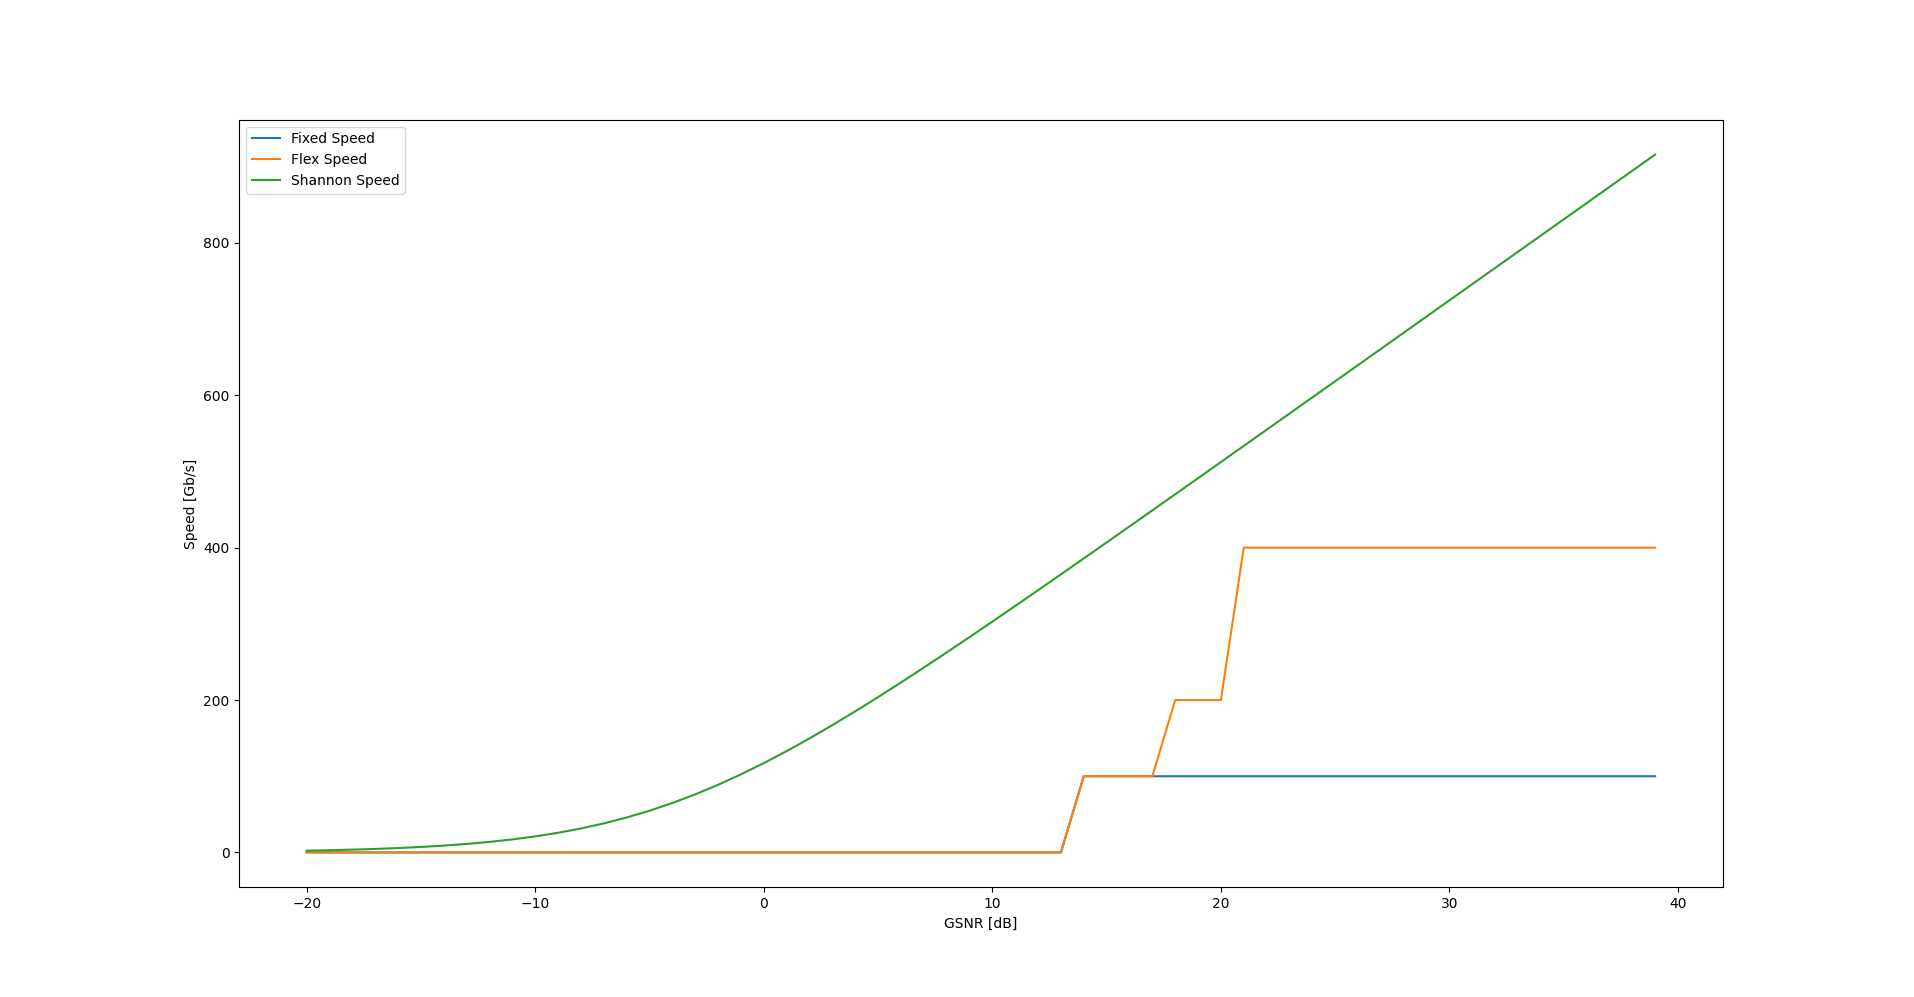
\includegraphics[width=0.9\linewidth]{Pictures/speeds achivable.png}
			\label{fig:trans_speed}
			\caption{Achivable speeds with respect to GSNR}
		\end{figure}
	\end{frame}
	\subsection{Line}
	\begin{frame}{Line outline}
		This class represents multimode optical fiber, in the contest of these simulation it will have 10 available modes, but the constructor allows to specify any number of available modes.
	\end{frame}
	\begin{frame}{Line Attributes}
		The line class contains the following attributes:
		\begin{itemize}
			\item Label: the name of the line that is the name of the beginning node followed by the end node.
			\item Length: the length of the line calculated from the position of the nodes at the beggining and end of the line
			\item State: a list which contains a string for each channel of the line which indicates if it is occupied or not by a light path.
			\item  Successive: a dictionary which contains the references to the begin and end node of the line which are identified by 'begin' and 'end' strings respectivly.
			\item In\_Service: a boolean value indicating if the line is working corectly or is damaged
		\end{itemize}
	\end{frame}
	\begin{frame}
		This class also implements two methods to calculate both linear and non linear noise introduced by the fiber itself and the amplifiers: \pause
		\begin{equation} % self.n_amplifiers * (cs.h * my_cs.BN * 10**(self.noise_figure/10) * (10**(self.gain/10) - 1) * self.f)
			P_{ase} = N_{amp} \cdot h \cdot B_n \cdot 10^{\frac{N_f}{10}} \cdot \left(10^{\frac{G}{10}} - 1 \right) \cdot f 
			\label{eq:P_ase}
		\end{equation} \pause
		\begin{equation}
			P_{nli} = P_{S}^3 \cdot \eta_{nli} \cdot B_n \cdot 10^{-\frac{\alpha_{dB} \cdot L}{10}} \cdot 10^{\frac{G}{10}}
			\label{eq:P_nli}
		\end{equation}
	\end{frame}
	%alpha = np.abs(self.alpha / (10 * np.log10(cs.e)))
	%log_arg = cs.pi**2 * self.module_beta * self.Rs**2 * len(self.state)**(2 * self.Rs/self.df)/(2* alpha)  # argument of log
	%factor = 16/(27 * cs.pi) * self.gamma**2 / (4 * alpha * self.module_beta * self.Rs**3)     # the other factor
	\begin{frame}
		The value of the constant $\eta_{nli}$ is calculated in the following way:
		\begin{equation}
			\eta_{nli} = \frac{16}{27\pi} \cdot \gamma^2 \cdot \frac{1}{4 \cdot \alpha \cdot \beta_2 \cdot R_s^3} \cdot log\left(\frac{\pi^2 \cdot \left|\beta_2\right| \cdot R_s^2 \cdot N_{ch}^{\frac{2 \cdot R_s}{\delta f}}}{2 \cdot \alpha}\right)
			\label{eq:eta_nli}
		\end{equation}
		where:
		\begin{equation}
			\alpha = \frac{\alpha_{dB}}{10 \cdot log_{10}\left(e\right)}
			\label{eq:alpha}
		\end{equation}
	\end{frame}
	\begin{frame}
		There is also a function to calculate the optimun launch power that generates the maximum GSNR:
		\begin{equation} % (80e3*self.noise_figure*(cs.h * my_cs.BN * self.f) / (2*my_cs.BN*self.calculate_NLI_coeff()))**(1/3)
			P_{opt} = \sqrt[3]{ L_{line} \cdot N_f \cdot \frac{h\cdot f}{2 \cdot \eta_{nli}}}
		\end{equation}
	\end{frame}
	\begin{frame}
		To calculate the latency occured by the signal traveling through the fiber line I used the foolowing formula:
		\begin{equation}
			\delta t = \frac{L_{line}}{c_{n}}
		\end{equation}
		Where $c_n$ is the speed of light in the optical medium, obtained by:
		\begin{equation}
			c_n = \frac{2}{3} \cdot c
		\end{equation}
	\end{frame}
	\subsection{Connetion}
	\begin{frame}{Connetion outline}
		This class represents a virtual circuit established between two nodes in the network, it contains all the data for that connection like the bit rate, the snr, and the channel.
	\end{frame}
	\begin{frame}{Influence of transceiver technology}
		Following are the graph resulting from 100 random connections between the node of the network topology shown in previous slides usign all the three possible transceivers technologies.
		\begin{figure}[h]
			\centering
			\begin{subfigure}{0.31\textwidth}
				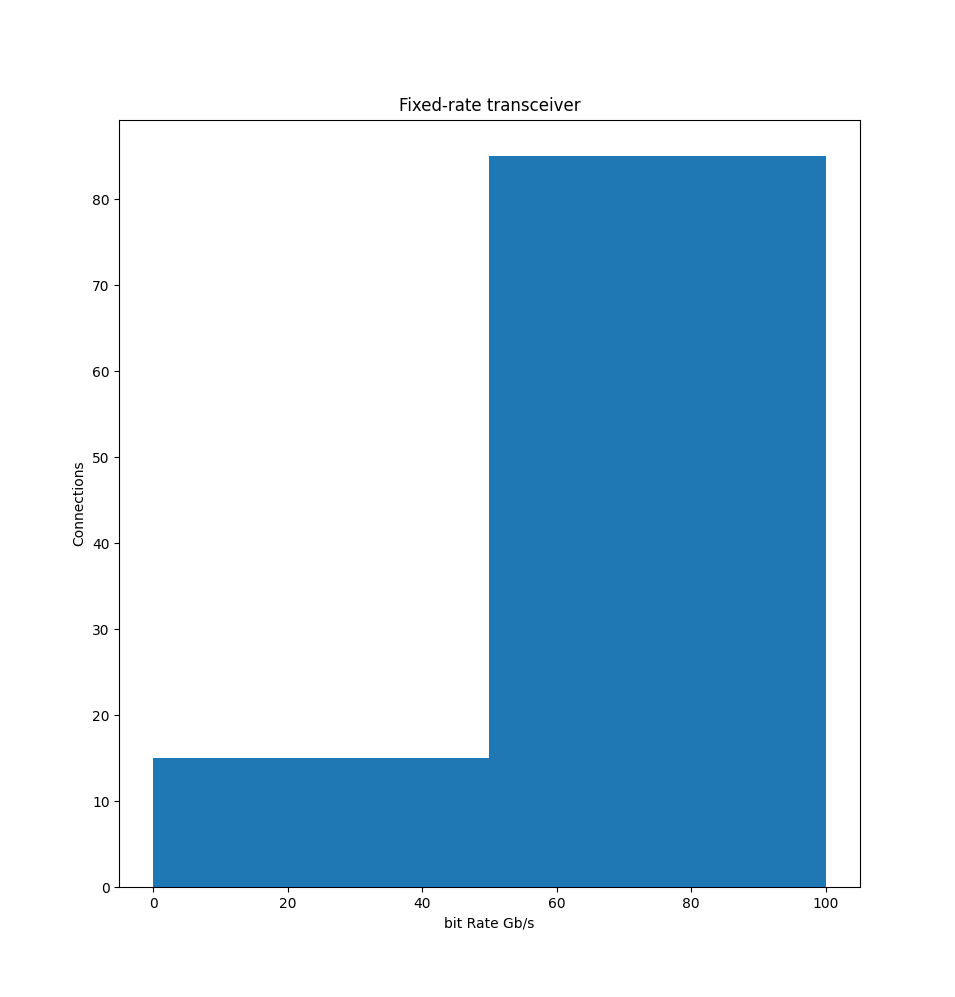
\includegraphics[width=\linewidth]{Pictures/Fixed rate cons.png}
				\caption{Fixed rate}
			\end{subfigure}
			\hspace*{\fill}
			\begin{subfigure}{0.31\textwidth}
				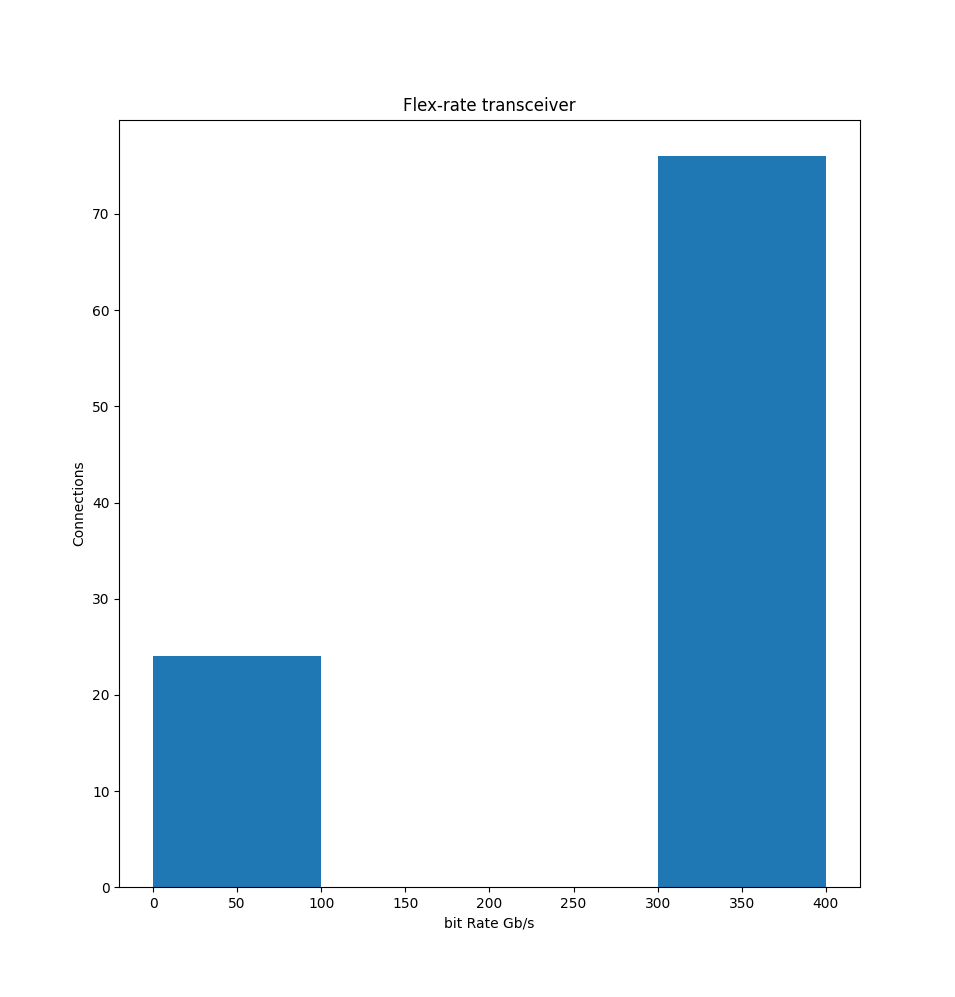
\includegraphics[width=\linewidth]{Pictures/Flex rate cons.png}
				\caption{Flex rate}
			\end{subfigure}
			\hspace*{\fill}
			\begin{subfigure}{0.31\textwidth}
				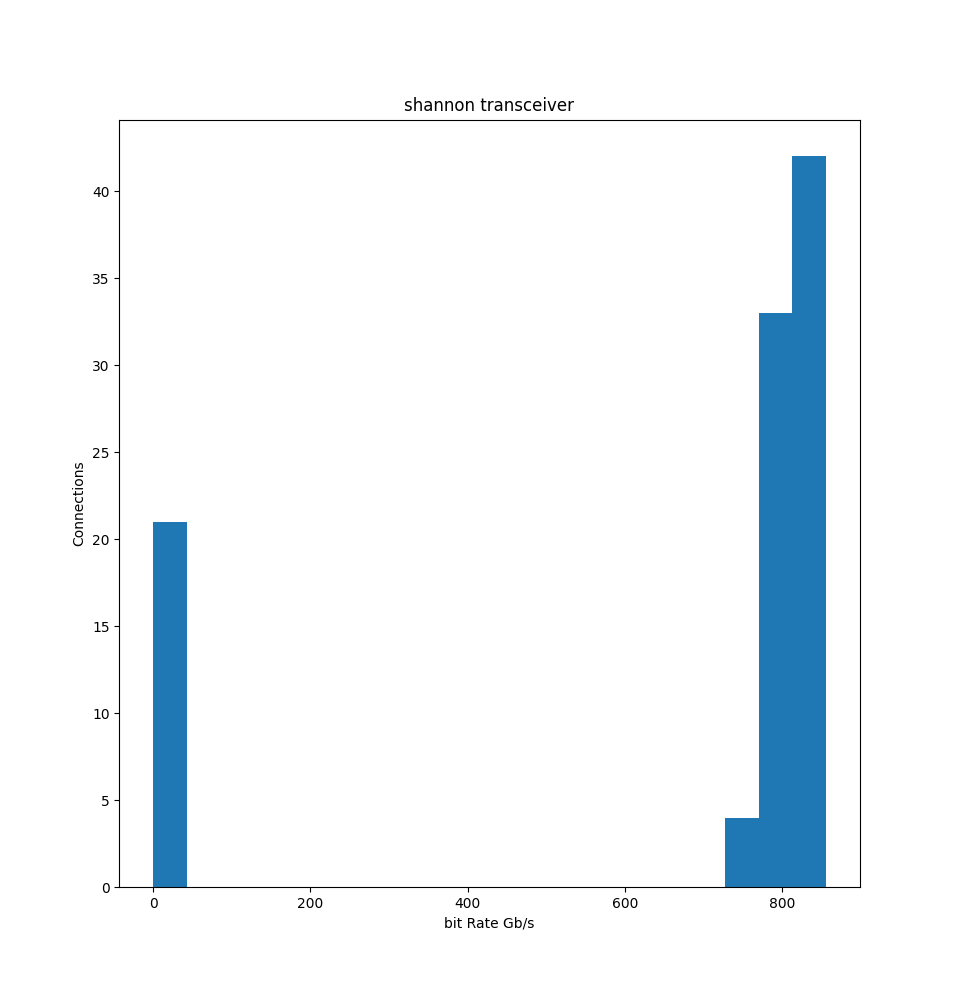
\includegraphics[width=\linewidth]{Pictures/shannon cons.png}
				\caption{Shannon}
			\end{subfigure}
		\end{figure}
	\end{frame}
	\begin{frame}{Influence of transceiver technology}
		Also from the same simulation I repoert the following data obtained from the accepted connections (Bit rate $>0$):\\
		
		\centering
		\begin{tabular}{|V{3cm}|V{3cm}|V{3cm}|V{3cm}|}
			\hline Technology & Average speed [Gb/s] & Average GSNR [dB] & Average latency [ms] \\
			\hline Fixed rate & 100 & 34,25 & 2,63 \\
			\hline Flex rate & 400 & 34,06 & 2,75 \\
			\hline Shannon & 814 & 34,19 & 2,67 \\ 
			\hline
		\end{tabular}
	\end{frame}
	\begin{frame}{Refused connection}
		Since this network only implements CDC switches the blocking event that cause a connection to be refused are of two possible types:
		\begin{itemize}
			\item There is no continuity of wavelength through all of the availabe path.
			\item The path that garanties the continuity of wavelength do not satisfy the GSNR requirments of the transceiver.
		\end{itemize}
	\end{frame}
	\section{Network class}
	\begin{frame}{Network class outline}
		This is the main class of the moduled I developed it is able to load the network topology from a json file and it is able to emulate the physical layer of the network.% cambia qua
	\end{frame}
	\begin{frame}{Main attributes}
		This class has the following main attributes:
		\begin{itemize}
			\item weighted\_paths: it is a panda data frame that contains the noise power, the latency and the GSNR for each possible possible light path.
			\item route\_space: it is a panda data frame that contains for each possible path through the network the list of available channels.
			\item logger: it is panda data frame that contains the list of created lightpaths, each with the time at which it was created, the path through the network and the bitrate.
		\end{itemize}
	\end{frame}
	\begin{frame}{Main methods}
		The main methods of this class are:
		\begin{itemize}
			\item Stream: given a list of connections it tries to fullfil them all selecting the best path for either GSNR or latency.
			\item manageTrafficMatrix: given a traffic matrix as input it selects start and end nodes randomly and tries to satifies the traffic request between the two; it continues untill it can longer satisfy any request.
			\item traffic\_recovery: it allowes the network to check all the connection it established and registered in the logger against the "physical" state of the lines for any discrepancies. If it finds any it tries to create new connections to satisfy the same traffic demand.
		\end{itemize}
	\end{frame}
	\begin{frame}{Total capacity of the network}
		I then tried for each of the three possible transceivers technologies to submit the a traffic matrix generated  in the following way(the unit is bit/s):
		\begin{equation} \label{eq:T}
			T_{ij} = \begin{cases}
				m \cdot 100 \cdot 10^9 $\hspace{10px} if $ i \neq j \\
				0$\hspace{61px} if $ i = j
			\end{cases}
		\end{equation} 
		where m is an integer value.\pause \\
		After submtting the matrix to the network I then calculated the allocated capacity using the following formula:
		\begin{equation}
			C = \frac{\sum_{1}^{N_{lines}} N_{Och}}{\left(N_{lines} - N_{damaged}\right) \cdot N_{Tch}} \cdot 100
		\end{equation}\pause
		Finally I simulated a fault (like a fiber cut) on the most congest line and called the traffic\_recovery method and then measured the allocated capacity again.
	\end{frame}
	\begin{frame}{Simulations results}
		I ran the simulation varying m from 0 to 80.
		\begin{figure}
			\begin{subfigure}{0.31\textwidth}
				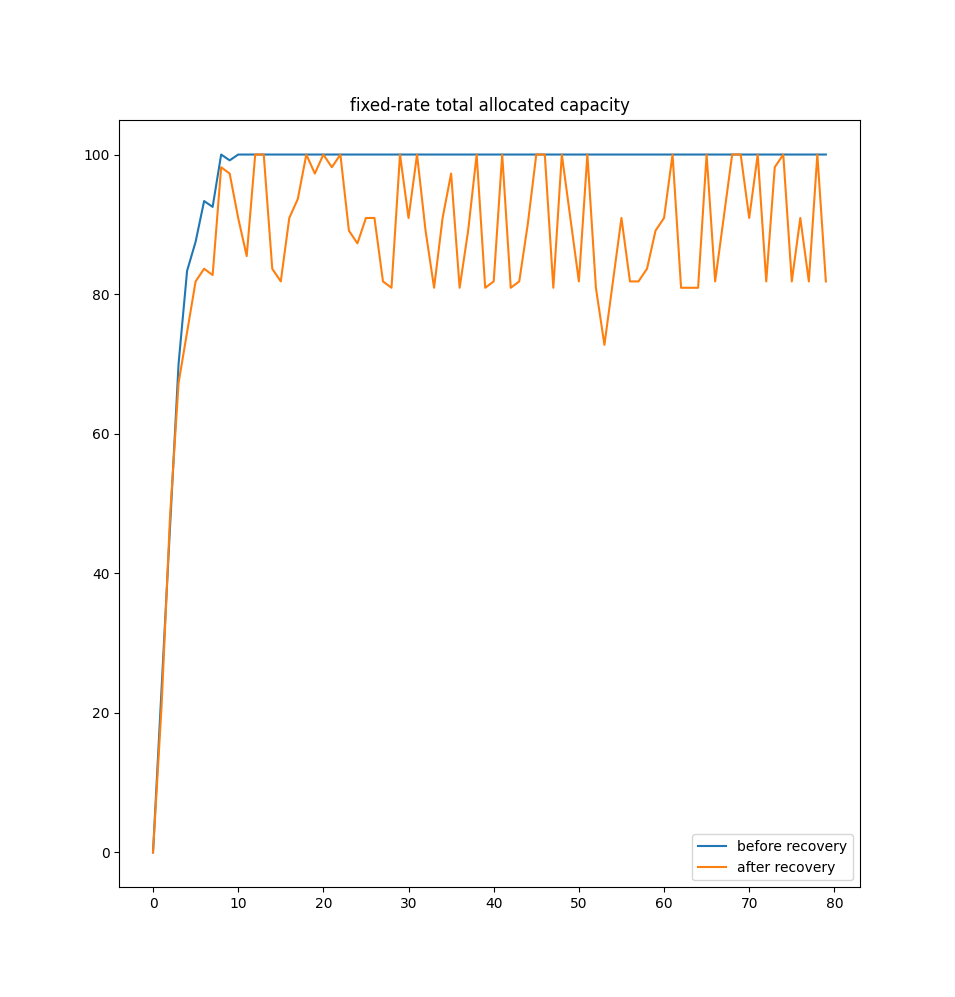
\includegraphics[width=\linewidth]{Pictures/fixed rate capacity.png}
				\caption{fixed rate}
			\end{subfigure}
			\hspace*{\fill}
			\begin{subfigure}{0.31\textwidth}
				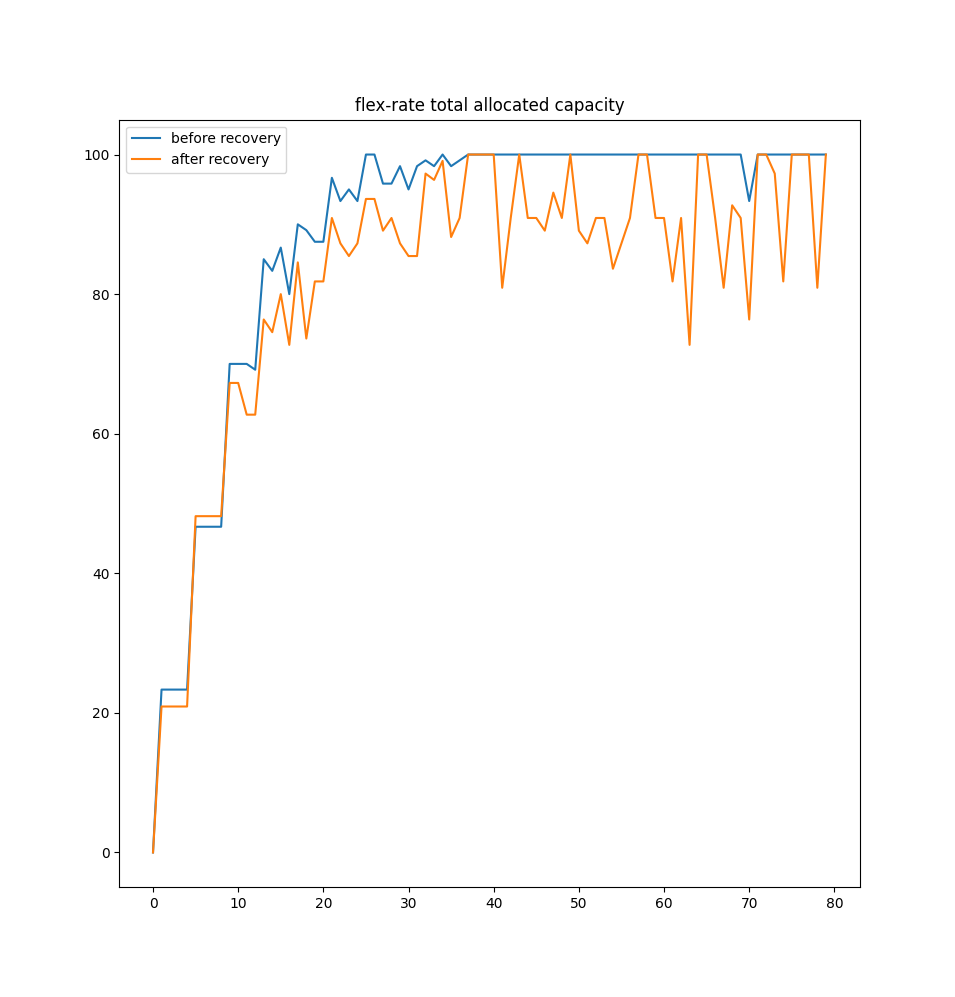
\includegraphics[width=\linewidth]{Pictures/flex rate capacity.png}
				\caption{flex rate}
			\end{subfigure}
			\hspace*{\fill}
			\begin{subfigure}{0.31\textwidth}
				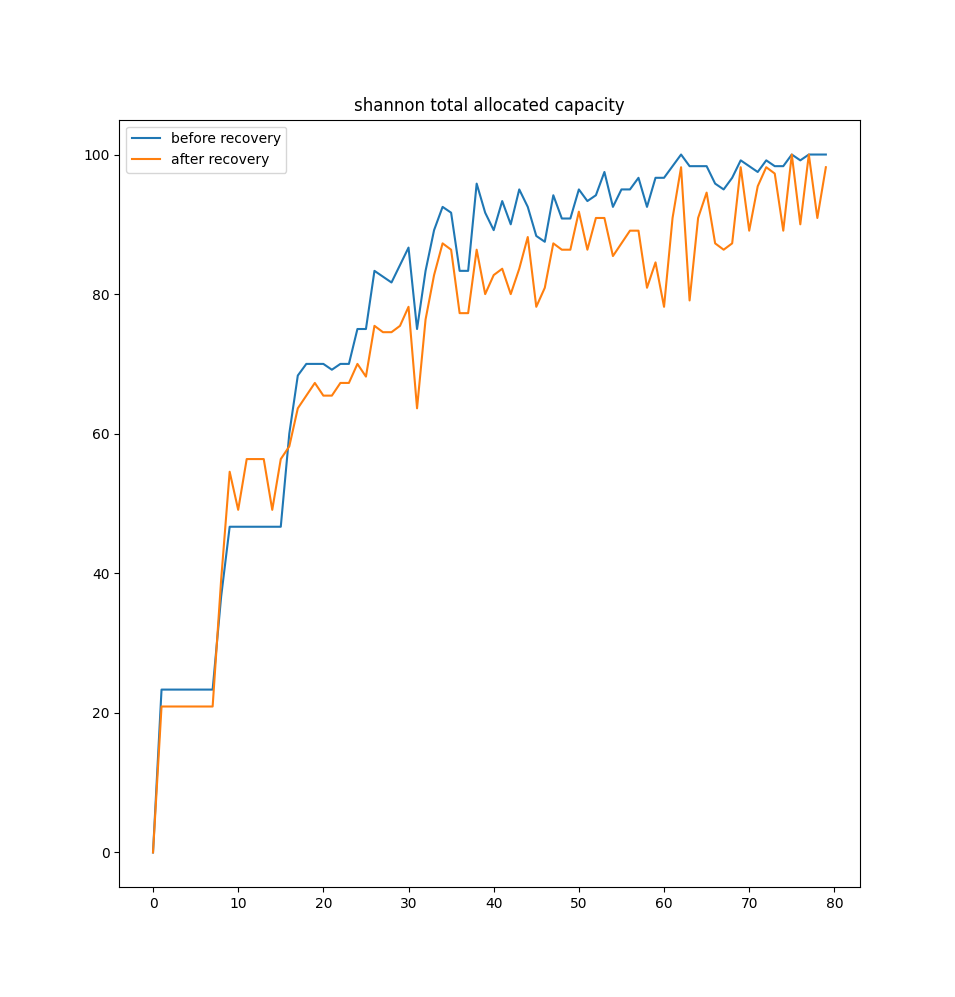
\includegraphics[width=\linewidth]{Pictures/shannon capacity.png}
				\caption{shannon}
			\end{subfigure}
		\end{figure}
	\end{frame}
	\begin{frame}{Simulation results}
		As we can see from the images the fixed rate the network allocates all the available capacity with a traffic matrix requiring $10 \cdot 100$ Gb/s 
		since the maximum speed on any channel  is $100$ Gb/s and there are 10 channels per fiber ottic that is the maximum amount of data that can pass for each fiber optic cable.\pause\\
		Similarly it is possible to observe that the flex rate network reaches maximum allocated capacity when the request to and from each node is $40 \cdot 100$ Gb/s for the same reason;\pause\\
		This is also true for the shannon network which only reaches that sate at $80 \cdot 100$ Gb/s.
	\end{frame}
	\begin{frame}
		Another way to compare the result of the previous simulation can also be analised through the average snr of the light Path in the network:
		\begin{figure}[h]
			\centering
			\begin{subfigure}{0.31\textwidth}
				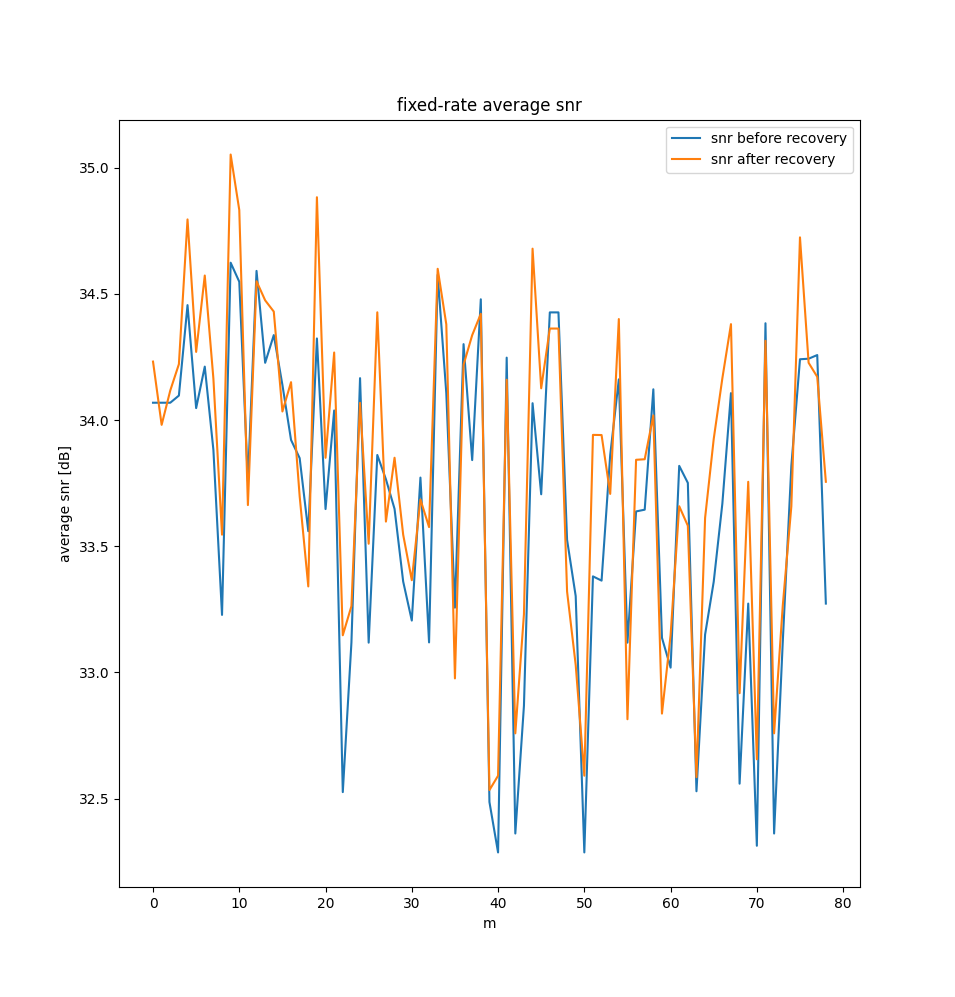
\includegraphics[width=\linewidth]{Pictures/fixed rate average snr.png}
				\caption{Fixed rate}
			\end{subfigure}
			\hspace*{\fill}
			\begin{subfigure}{0.31\textwidth}
				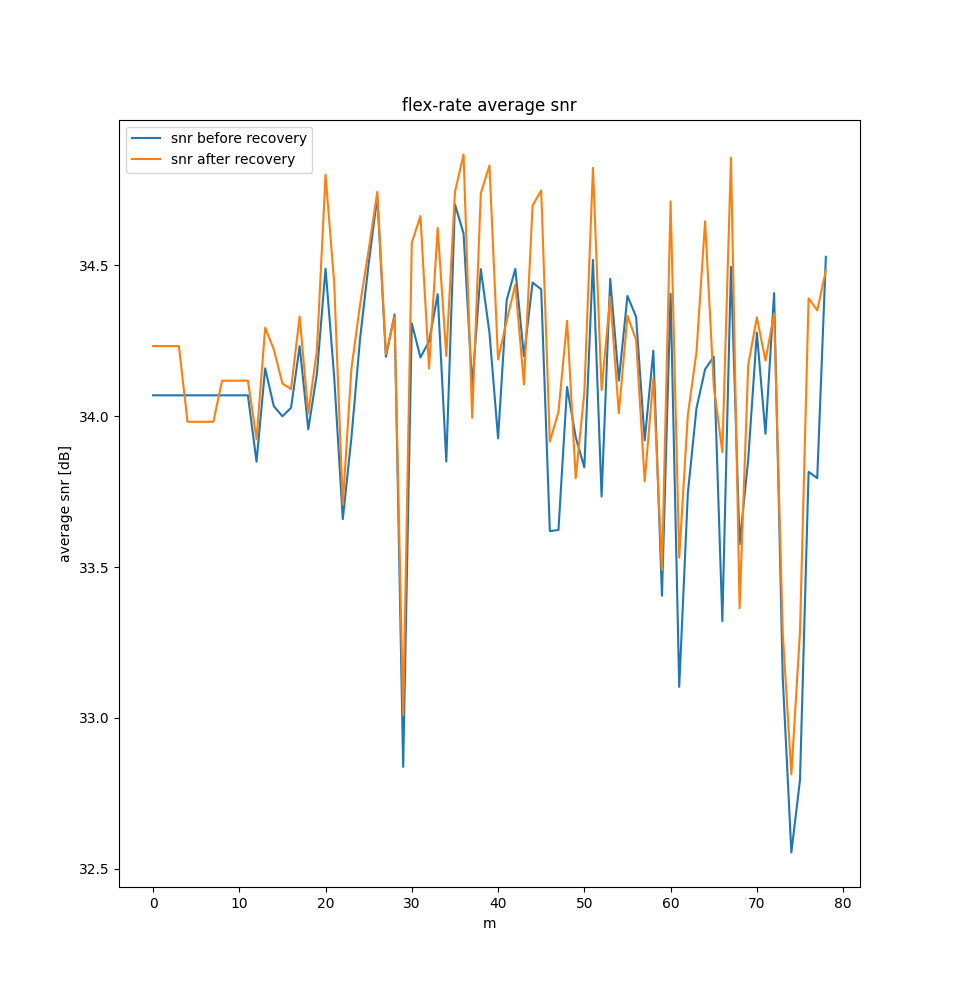
\includegraphics[width=\linewidth]{Pictures/flex rate average snr.png}
				\caption{Flex rate}
			\end{subfigure}
			\hspace*{\fill}
			\begin{subfigure}{0.31\textwidth}
				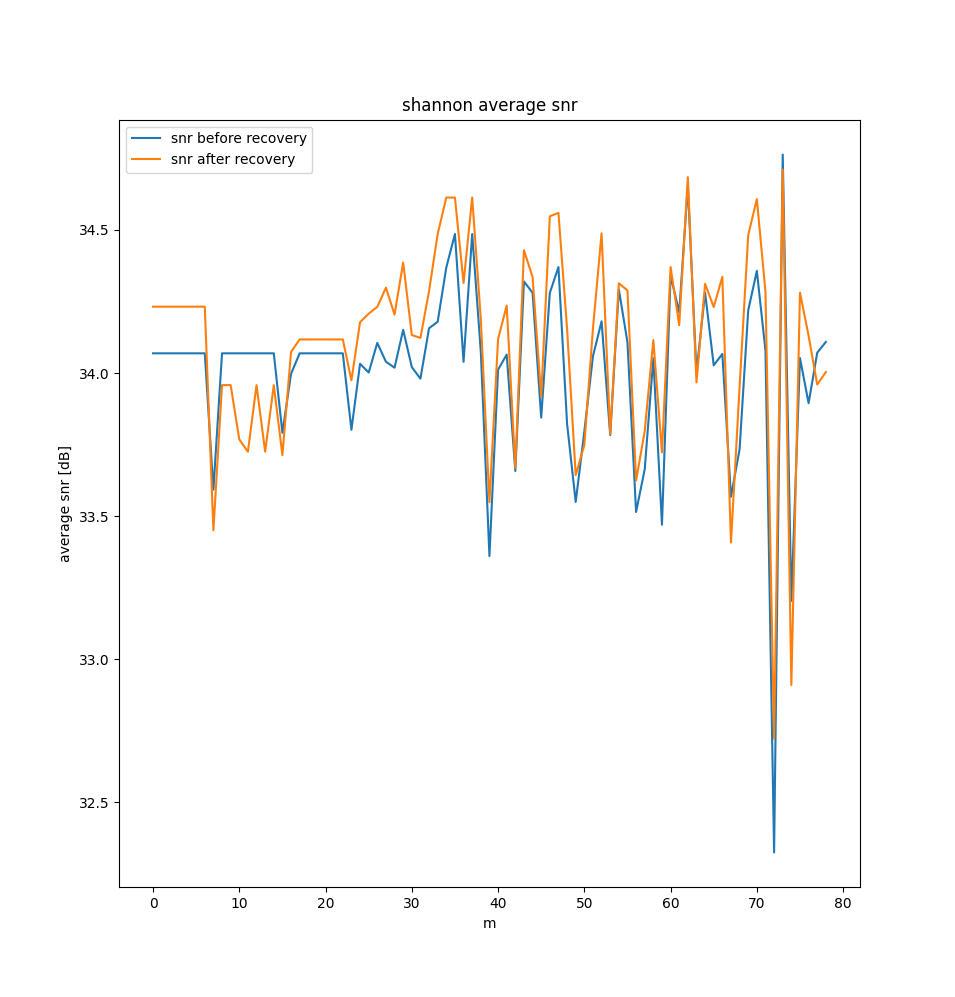
\includegraphics[width=\linewidth]{Pictures/shannon average snr.png}
				\caption{Shannon}
			\end{subfigure}
		\end{figure}
	\end{frame}
	\section{End}
	\begin{frame}
		\begin{Huge}
			\begin{center}
				Fin.
			\end{center}
		\end{Huge}
	\end{frame}
\end{document}